%-------------------------------------------------------
% HEADER
%-------------------------------------------------------

\documentclass[10pt, aspectratio=169]{beamer}
\usetheme[]{Feather}
 %Change the bar colors:
%\setbeamercolor{Feather}{fg=green!20,bg=green}
% Change the color of the structural elements:
%\setbeamercolor{structure}{fg=red}
% Change the frame title text color:
%\setbeamercolor{frametitle}{fg=blue}
% Change the normal text color background:
%\setbeamercolor{normal text}{fg=black,bg=gray!10}
\usepackage[utf8]{inputenc} %default packages
\usepackage[english]{babel}
\usepackage[T1]{fontenc}
\usepackage[scaled]{helvet}
\usefonttheme[onlymath]{serif} %For LaTeX-style looking equations
\usepackage{amsfonts} %default packages
\usepackage{amsmath}
\usepackage{amssymb}
\usepackage{amsthm}
\usepackage{amstext}
\usepackage{tikz} %making graphs within LaTeX
\usepackage{graphicx}
\usepackage{mathtools} %drawing picture with tikz
\usepackage{pgfplots} %making plots within LaTeX
\usepackage{pgfplotstable} %for importing data from csv files
\pgfplotsset{compat=1.17}
\usepackage{tabularx} %for tables centered
\usepackage{booktabs} %for better looking tables
\usepackage{longtable}
\usepackage{subcaption} % provides subfigures within figures 
\usepackage[absolute,overlay]{textpos} %for placing figures wherever
\usepackage{animate} %for making GIF animations
%small font size for the bibliography at the end
\newcommand\Fontvi{\fontsize{6}{7.2}\selectfont}


%-------------------------------------------------------
% INFORMATION IN THE TITLE PAGE
%-------------------------------------------------------

\title[] % [] is optional - is placed on the bottom of the sidebar on every slide
{ % is placed on the title page
      \textbf{851-0101-86 S Complex Social Systems: Modeling Agents, Learning, and Games}
}

\subtitle[]
{
      \textbf{Crop Wars: Agent-based simulation of agricultural interactions}
}

\author[]
{      Christopher Golling, Gael Mourouga, Aaron Moser, Otto Schmidt, Amir H. Keshavarzzadeh
      {}
}

\institute[]
{
      %GDR redox-flow
  
  %there must be an empty line above this line - otherwise some unwanted space is added between the university and the country (I do not know why;( )
}

\date{}

%Programatically defining the sections to be called on the slides title
\def\a{Different types of frames with LaTeX}
\def\aa{Basic frames}
\def\aaa{Text and maths}
\def\aab{Image}
\def\aac{Image and text}
\def\ab{More advanced frames}
\def\aba{Animation on click}
\def\abb{GIF animation}

%-------------------------------------------------------
% START OF DOCUMENT
%-------------------------------------------------------

\begin{document}

%-------------------------------------------------------
% THE TITLEPAGE
%-------------------------------------------------------

{\1% % this is the name of the PDF file for the background
\begin{frame}[plain,noframenumbering] % the plain option removes the header from the title page, noframenumbering removes the numbering of this frame only
  \titlepage % call the title page information from above
\end{frame}}


\begin{frame}{Content}{}
    \tableofcontents
\end{frame}

%-------------------------------------------------------
\section{\a}
%-------------------------------------------------------

\subsection{\aa}
%-------------------------------------------------------

\subsubsection{\aaa}
\begin{frame}{\aa}{\aaa}
    text:
\begin{equation}
    U = \sum_i a_k c^k
\end{equation}
\end{frame}

\subsubsection{\aab}
\begin{frame}{\aa}{\aab}
    \begin{figure}
      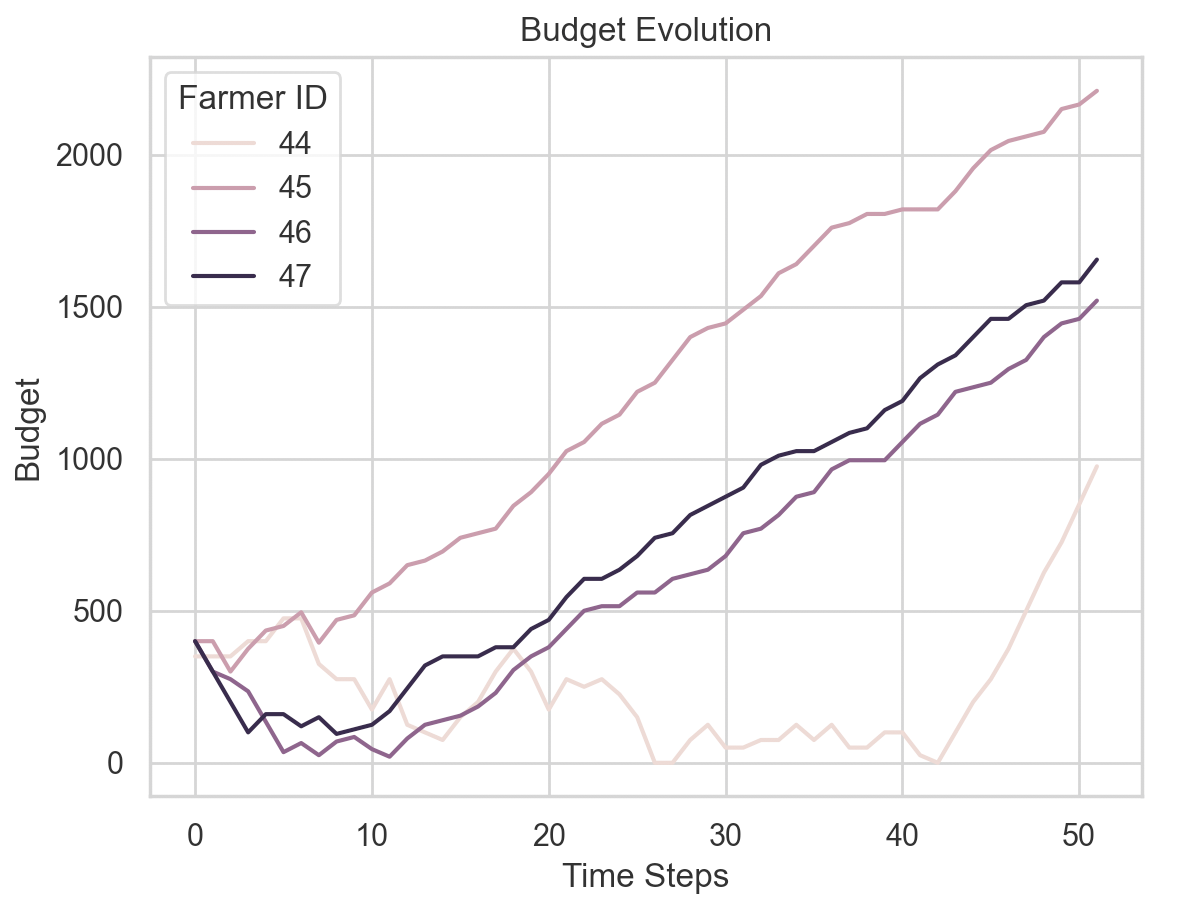
\includegraphics[scale=0.45]{Figures/v12_Budget.png}
    \end{figure}
\end{frame}

\subsubsection{\aac}
\begin{frame}{\aa}{\aac}
    \begin{columns}
      \column{0.48\linewidth}
         \centering
         \begin{figure}
          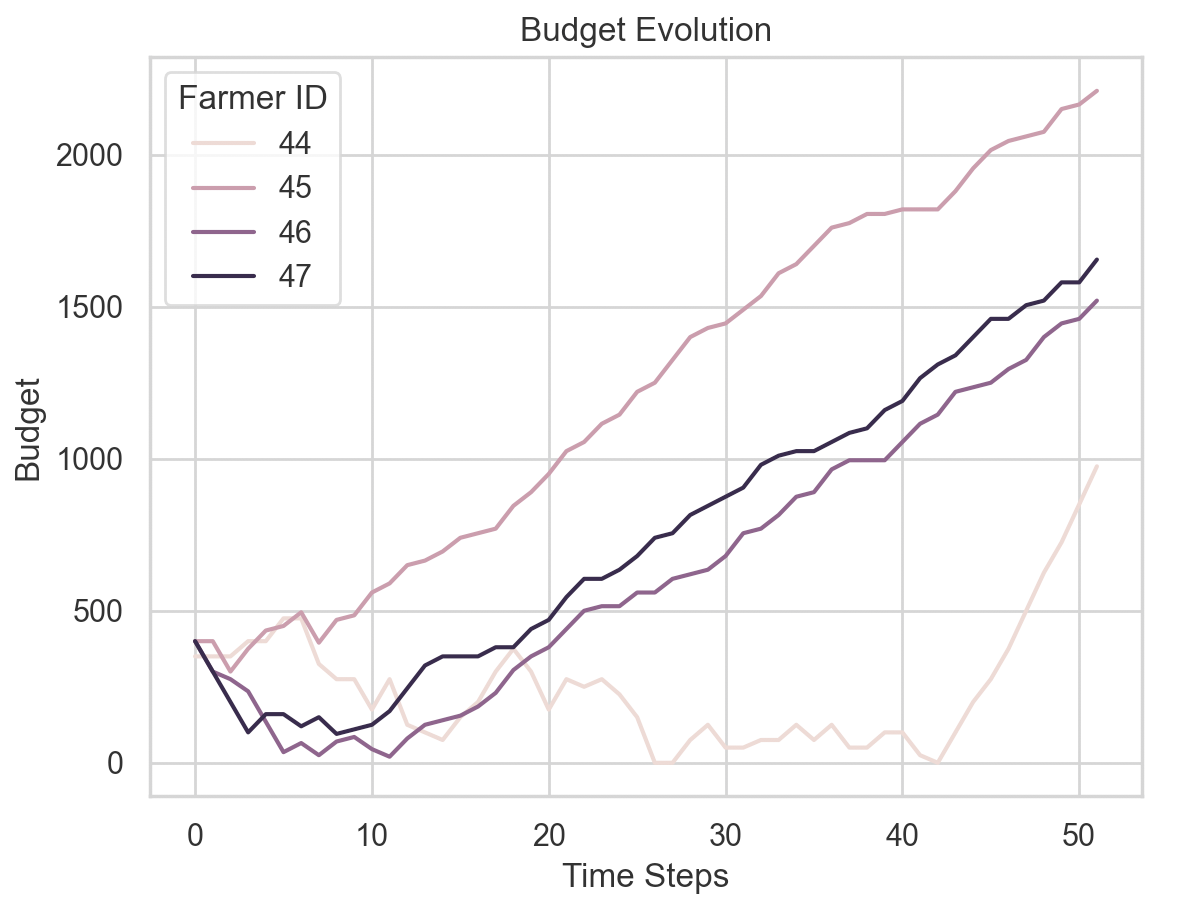
\includegraphics[scale=0.30]{Figures/v12_Budget.png}
         \end{figure}
       \column{0.52\linewidth}
       Text:
       \begin{equation}
        \phi \approx \frac{a}{b} \ln \left( \frac{a}{b} \right)
      \end{equation}
     \end{columns} 
\end{frame}

\subsection{\ab}

\subsubsection{\aba}
\begin{frame}{\ab}{\aba}
    \begin{itemize}
        \item<1-> point 1
        \item<2-> point 2
        \item<3-> point 3
        \item<4-> point 4
    \end{itemize}
\end{frame}

\subsubsection{\abb}
\begin{frame}{\ab}{\abb}
    \centering
    \animategraphics[loop,width=4cm]{10}{Figures/ThankYouGIF/frame-}{0}{6}
\end{frame}

\end{document}

